\subsubsection{照度センサー}\label{light}
\begin{table}[H]
	\begin{tabular}{|p{\colF}|p{\colG}|}	\hline
	名称 & 照度センサー(しょうどせんさー)\\ \hline
	接続箇所 & アナログコネクタ (3pin)\\ \hline
	機能概要 & 周辺の明るさの測定\\ \hline
  \end{tabular}
\end{table}

\begin{table}[H]
	\begin{tabular}{|p{\colF}|p{\colG}|}	\hline
	サンプルコードの場所 & 05/anain.hsp\\ \hline
	raspiへの入力 & 明るさを表す0から1023の値。明るいと値が減り、暗いと値が増える。\\ \hline
	raspiへの入力方法 & val = gpioin(GPIO番号)\\ \hline
	raspiからの出力 & なし\\ \hline
	raspiからの出力方法 & なし\\ \hline
  \end{tabular}
\end{table}

\begin{table}[H]
	\begin{tabular}{|p{\colF}|p{\colG}|} \hline
	使い道 & 照度計測、カメラの\ruby{露出}{ろ|しゅつ}調節機能に。\\ \hline
	注意事項 & 材料の\ruby{硫化}{りゅう|か}カドミウム(CdS)は人体に有害なため、\ruby{割}{わ}れたセンサーを素手で触らないこと。\\ \hline
	補足 & なし\\ \hline
  \end{tabular}
\end{table}

\begin{figure}[H]
	\begin{tabular}{|p{\colH}|p{\colI}|p{\colH}|p{\colI}|} \hline
	外観 & 
	\begin{minipage}[t]{\linewidth}
    \smallskip
      \centering
      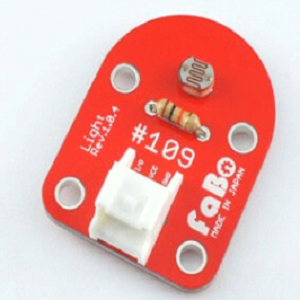
\includegraphics[width=\linewidth]{images/chap05/text05-img024.png}
      \caption{照度センサー}
      \smallskip
    \end{minipage} &
    回路記号 & 
    \begin{minipage}[t]{\linewidth}
    \smallskip
      \centering
      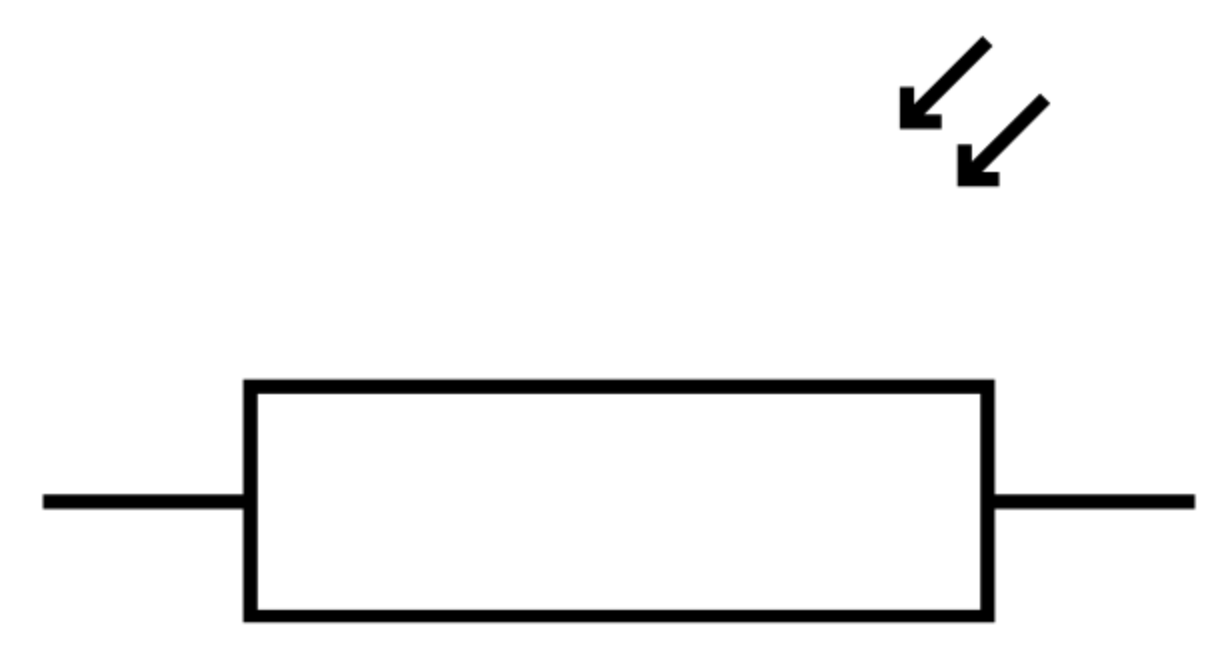
\includegraphics[width=\linewidth]{images/chap05/text05-img053.png}
      \caption{照度センサーの回路図}
      \smallskip
    \end{minipage}\\ \hline
  \end{tabular}
\end{figure}
